\section{Bulk Loading Process}
\vspace{-0.2cm}
%The bulk loading phase is the most important feature of the framework for it completes the division of index partitions and construction of index. As such, we now discuss this facet of the framework in greater detail.
The bulk loading phase has three stages, including local index construction, index partition division and global index construction. Firstly, each data node builds its own local index and sends statistic information of search keys to the coordinator. Secondly, the coordinator generates multiple uniform ranges on search keys based on statistic information from data nodes, and sends the ranges to corresponding data nodes. Finally, data nodes receive ranges from the coordinator create index partitions by shuffling data. Note that Algorithm 1 is the main program. Algorithm 1 calls local index construction routine (Algorithm 2), index partition division routine (Algorithm 3) and global index construction (Algorithm 4) routine in proper order.

Algorithm 1 illustrates the framework of the bulk loading approach in distributed LSM-tree data stores. We assume we will construct a secondary index on column search\_key of table $T$. And partitions $P$ of table $T$ are distributed to multiple data nodes. So, all data nodes contained $p\in P$  run the function RunLocalIndex(p, interval,serach\_key, storing) (Algorithm 2) to build local index and report the histogram $H$ containing search\_key distribution information to the coordinator (at line 6). Afterwards, the coordinator runs RunPartitionDivision(H,N) (Algorithm 3) to get balanced index data partitions based on histogram $H$ and the number of partitions of index data (at line 9), and assigns partition ranges to appropriate data nodes (at line 10). Finally, the data nodes receive range information from the coordinator and run RunGlobalIndex(L) (Algorithm 4) to build the global index based on index partition range list $L$ (at line 12).


\SetKwProg{Fn}{\underline{}}{}{end}
\newcommand{\forcond}{$i=0$ \KwTo $n$}
\SetKwFunction{localindexconstruct}{RunLocalIndex}
\SetKwFunction{globalindexconstruct}{RunGlobalIndex}
\SetKwFunction{firstsampling}{RunLocalSampling}
\SetKwFunction{sampling}{RunPartitionDivision}
\SetKwFunction{indexrequest}{RunIndexRequest}
\SetKwFunction{secondsampling}{RunpartitionSampling}
%\SetAlgorithmName{Figure}{}
\LinesNumbered
\newcommand{\fortol}{$i=0$ \KwTo $L$}
\newcommand{\fortok}{$j=1$ \KwTo $k$}
\vspace{-0.5cm}
\begin{algorithm}[htb]
	\SetAlgoLined
	\caption{Index Bulk Loading}%
	Let $P$ denote partition set of table $T$ which needs to construct index\;
	Let $h_i$ and $H$ denote a bucket and an array of equi-depth histogram respectively\;
	Let $R$ denote an array of range
	\tcc{construct local index}
	%\ForEach{$SN$}
	%{
	\ForEach{partition $p \in P$ in all data nodes}
	{
		%$(local\_index,h_i) \leftarrow$ {\localindexconstruct{p,depth}} \;
		$h_i\leftarrow$ {\localindexconstruct{p, depth}} \;
		%add $histogram$ to histogram array $H$\;
		$H.add(h_i)$\;
	}
	report $H$ to Coordinator\;
	%}
	\tcc{divide index partition range}
	$R \leftarrow$ {\sampling{H, N}} \;
	Coordinator sends the partition range $R[i]$ to all data node  with respect to $R[i]$ \;
	\tcc{construct index partition}
	\ForEach{$data node$ correlated to $R[i]$}
	{
		$index\_partition \leftarrow$ \globalindexconstruct{R[i]}\;
		%   add $index\_partition$ info to array $report\_info$\;
	}
	
\end{algorithm}
\vspace{-0.5cm}
 %A covering index is an index that contains all, and possibly more, the columns you need for your query
 \vspace{-0.2cm}
 \subsection{Local Index Construction}
Local index construction starts after the initialization phase. Algorithm 2 illustrates the process of local index construction. Note that Algorithm 2 must run at data nodes. Each data node scans the original data table partitions located in itself in order to construct index entries (at lines 6-14). If we need to build the covering index, i.e. storing columns are not NULL, an index entry needs to contain storing columns besides the search key and primary key of the original table (at line 8). Otherwise, an index entry only contains the search key and primary key (at line 11). And an equi-depth histogram $H_i$ is adopted to capture data distributions on search keys, where each bucket is defined by an interval which is left-closed and right-open, i.e. $[start\_key, end\_key)$ (at lines 15-26). And $interval$ represents the depth of the bucket $h$. The size of depth of bucket can be adjusted. Smaller bucket depth means more accurate information of data distributions, but it also needs more space to store more statics information. Finally, the local index records are written to the disk (at line 25).


\SetKwProg{Fn}{\underline{Function}}{}{end}
%        \newcommand{\forcond}{$i=0$ \KwTo $n$}
\SetKwFunction{localindexconstruct}{RunLocalIndex}
\SetKwFunction{globalindexconstruct}{RunGloalIndex}
%\SetAlgorithmName{Figure}{}
\LinesNumbered
%           \newcommand{\fortol}{$i=0$ \KwTo $L$}
%           \newcommand{\fortok}{$j=1$ \KwTo $k$}
\vspace{-0.5cm}
\begin{algorithm}[htb]
	\SetAlgoLined
	\caption{RunLocalIndex}%
	%\Fn(\tcc*[h]{handle request for index records}){\indexrequest{range}}
	\Fn(\tcc*[h]{local index construction}){\localindexconstruct{P, search\_key, storing}}{	
		Let $r$ and $r'$  denote a record of data table and index table respectively \;
		Let $P'$ denote the set of index records sorted by search\_key \;
		Let $H$ and $h[j]$ denote a equi-depth histogram and a bucket respectively \;
		int $i, j\leftarrow 0$; $P' \leftarrow \emptyset$; $Flag \leftarrow TRUE$ \;
		%bool $is\_start\_key \leftarrow $ true\;
		\For{each $r \in P$}
		{
			\If {storing is NULL}
			{
				$r' \leftarrow (r.search\_key, r.primary\_key, storing ) $ \;
			}
			\Else
			{
				$r' \leftarrow (r.search\_key, r.primary\_key)$\;
			}
			$P' \leftarrow  P'$ inserted $r'$ based on the order of search-key   \;
		}
		%\For{each $r' \in P'$}
		%$h[1].start\_key \leftarrow r'[1].search\_key$ \;
		\While{$i <> |P'|$}
		{
			i++ \;
			\If {Flag}
			{
				$h[j].start\_key \leftarrow r'[i-1].search\_key$ ; $Flag \leftarrow FALSE$  \;
			}
			\If {$i$ mod $interval ==0$}
			{
				$h[j].end\_key \leftarrow r'[i].search\_key$ \;
				$Flag \leftarrow TRUE$;  j++\;
				$H \leftarrow H \cup h[j]$ \;
			}
			%  i++ ;
			write $r'$ to local index partition on disk \;
		}
		\Return$H$
		%  Report $h_i$ to the coordinator \;
	}
\end{algorithm}
\vspace{-0.5cm}

\begin{example}
To help explain this process, we refer to Figure 4 as our running example. Table Item has 16 records and contains three partitions, i.e. partition1, partition2 and partition3 on DataNode1, DataNode2.
Local index construction in Figure 4 describes the process local index construction. Each record in a partition is mapped to an index record and index records are sorted by the primary key of the index table. In our example, the primary key of the index table is ($Sale,Item\_Id$). After local index construction, three $local\_indexes$ $local\_index1$, $local\_index2$, $local\_index3$ are constructed.  The equal-depth histogram of partition1 is shown in Figure 5. The depth of bucket is 2. Thus three buckets are sampled. As $<(101,3001),(201,3002)>$, $<(201,3002),(400,3004)>$ and $<(400,3004),(600,3006)>$ in Figure 5. %×ó±ÕÓÒ¿ª
\end{example}

\vspace{-0.6cm}
\begin{figure}
	\hspace*{-6mm}
	\includegraphics[width=13cm]{articlegraph/index_example.pdf}
	\caption{Index Bulk Loading}
\end{figure}
\vspace{-0.6cm}

\vspace{-0.2cm}
\subsection{Balanced Index Partition Division}
After local index construction, the coordinator will receive equal-depth histograms of all $local\_index$ and then divide the index data into multiple uniform partitions. It is very important to decide the number of partitions and the division strategy of the index data. Subsequently, more details will be explored.

Generally, the larger size of partition means less efficient for high selective queries, while the smaller size of partition means more space for meta data in a distributed database.
Thus, we have to set an appropriate size of partition for the index data.
Considering a table T($col_1,col_2...col_n$) with an index I on $col_j$.  Let $size(T)$ and  $M$  denote the size of $T$ and the maximal limitation of partition size of $T$ respectively. In fact, the partition number $P$ of $T$ can be defined by Equation $(1)$. Similarly, the partition number of the index data on table $T$ denoted by $P'$ can be defined by Equation $(2)$.  The relationship between the number of index data partitions and the number of original data table partitions can be defined by Equation $(3)$. Furthermore, the index partition number can be calculated by Equation $(4)$ for fixed-length storage systems. However, we have to capture the size of index records during local index construction to calculate the partition number of the index by Equation $(2)$ for varying-length storage systems. In practice, we set the number of partitions of the index data same to the number of partitions of the original table data in order to reduce query response time.

\begin{align}
      & P= \frac{size(T)}{M}  \ (1)
      %&  N= \frac{size(I)}{M} \times rep\_num\ \ (2) \notag
      &  P'= \frac{size(I)}{M} \ \ (2) \notag
\end{align}
\begin{align}
      & P'= P \times \left( \frac{size(I)}{size(T)}\right)\ (3)
      & P'= P \times \left( \frac{size(search\_key, primary\_key)}{size(col_1, col_2 ... col_n)}\right) (4) \notag
\end{align}

Algorithm 3 illustrates the procedure where the coordinator divides the index data into multiple uniform partitions. So, Algorithm 3 must run at the coordinator node. First, the coordinator puts together a whole histogram $H'$ with the histogram $h_i$ received from each individual data node based on the order of  bucket (at line 5). Afterwards, The coordinator will divide the $H'$ into $ \lceil(|H'|-1)/N \lceil$  ranges, where $|H'|$ represents the number of buckets and $N$ is the number of index data partitions (at line 6). Note that each index data partition is defined by an interval [start\_key,end\_key) which is left-closed and right-open. Furthermore, the range is continuous, such as $(MIN, index\_key_1]$, $(index\_key_1, index\_key_2]$...$(index\_key_p, MAX)$. After the division, the coordinator will allocate ranges to data nodes and data nodes will construct corresponding partitions, which are described in the main program (Algorithm 1).
\SetKwProg{Fn}{\underline{Function}}{}{end}
% \newcommand{\forcond}{$i=0$ \KwTo $n$}
\SetKwFunction{firstsampling}{RunLocalSampling}
\SetKwFunction{secondsampling}{RunpartitionSampling}
\SetKwFunction{sampling}{RunPartitionDivision}
%\SetAlgorithmName{Figure}{}
\LinesNumbered
%\newcommand{\fortol}{$i=0$ \KwTo $L$}
% \newcommand{\fortok}{$j=1$ \KwTo $k$}
\vspace{-0.5cm}
\begin{algorithm}[!htb]
	%Let histogram be a structure that stores sampling info of a partition. Each sampling consists of rowkey pair: $(stary\_key,end\_key).$\;
	\SetAlgoLined
	\caption{RunPartitionDivision}%	
	\Fn{\sampling{H, N}}{
		Let $H'$ denote a equi-depth histogram which bucket is sorted by its start\_key \;
		Let $R$ denote an array of range defined by [start\_key, end\_key) \;
		Let $h[i]$ be the i-th bucket of $H'$ \;
		Load all buckets of $H$ based on the order of bucket.startkey into $H'$ \;
		$n \leftarrow \lceil(|H'|-1)/N\rceil$ \;
		$R \leftarrow \emptyset$; $i,j \leftarrow 0$; $Flag \leftarrow FALSE$  \;
		$R[1].start\_key \leftarrow h[1].start\_key$ \;
		%\For{each bucket $h[i] \in H'$}
		\While{$i <> |H'|$}
		{
			i++ \;
			\If {Flag}
			{
				$R[j].start\_key \leftarrow h[i-1].end\_key$; $Flag \leftarrow FALSE$  \;
			}
			\If{$i$ mod $n==0||i==|H'|$}
			{
				$R[j].end\_key \leftarrow h[i].end\_key$ \;
				$Flag \leftarrow TRUE$ ;
				j++ \;
			}
		}
		\Return R\;
	}
	
\end{algorithm}
\vspace{-0.5cm}

The key point of Algorithm 3 is to guarantee each data node maintains almost same size of the index, aiming at providing a good load balancing for query processing. The coordinator adopts two strategies to assign index ranges to data nodes: (1) \textbf{overlap priority}, it means that the coordinator assigns the index range to the data node which has maximal overlaps with the range. (2) \textbf{Load priority}, it means that the coordinator assigns the index range to the data node which has the lightest load. The overlap priority can reduce communication overhead, and the load priority can provide a quicker response for queries. The end users can adopt different policies according to application scenarios.
Certainly, the communication overhead cannot be totally avoided even when the overlap priority is adopted. Fortunately, communication overhead is generated in the offline stage. It has no effect on the response of query processing.

\vspace{-0.7cm}
\begin{figure}
	\begin{minipage}[t]{0.5\linewidth}
		\centering
		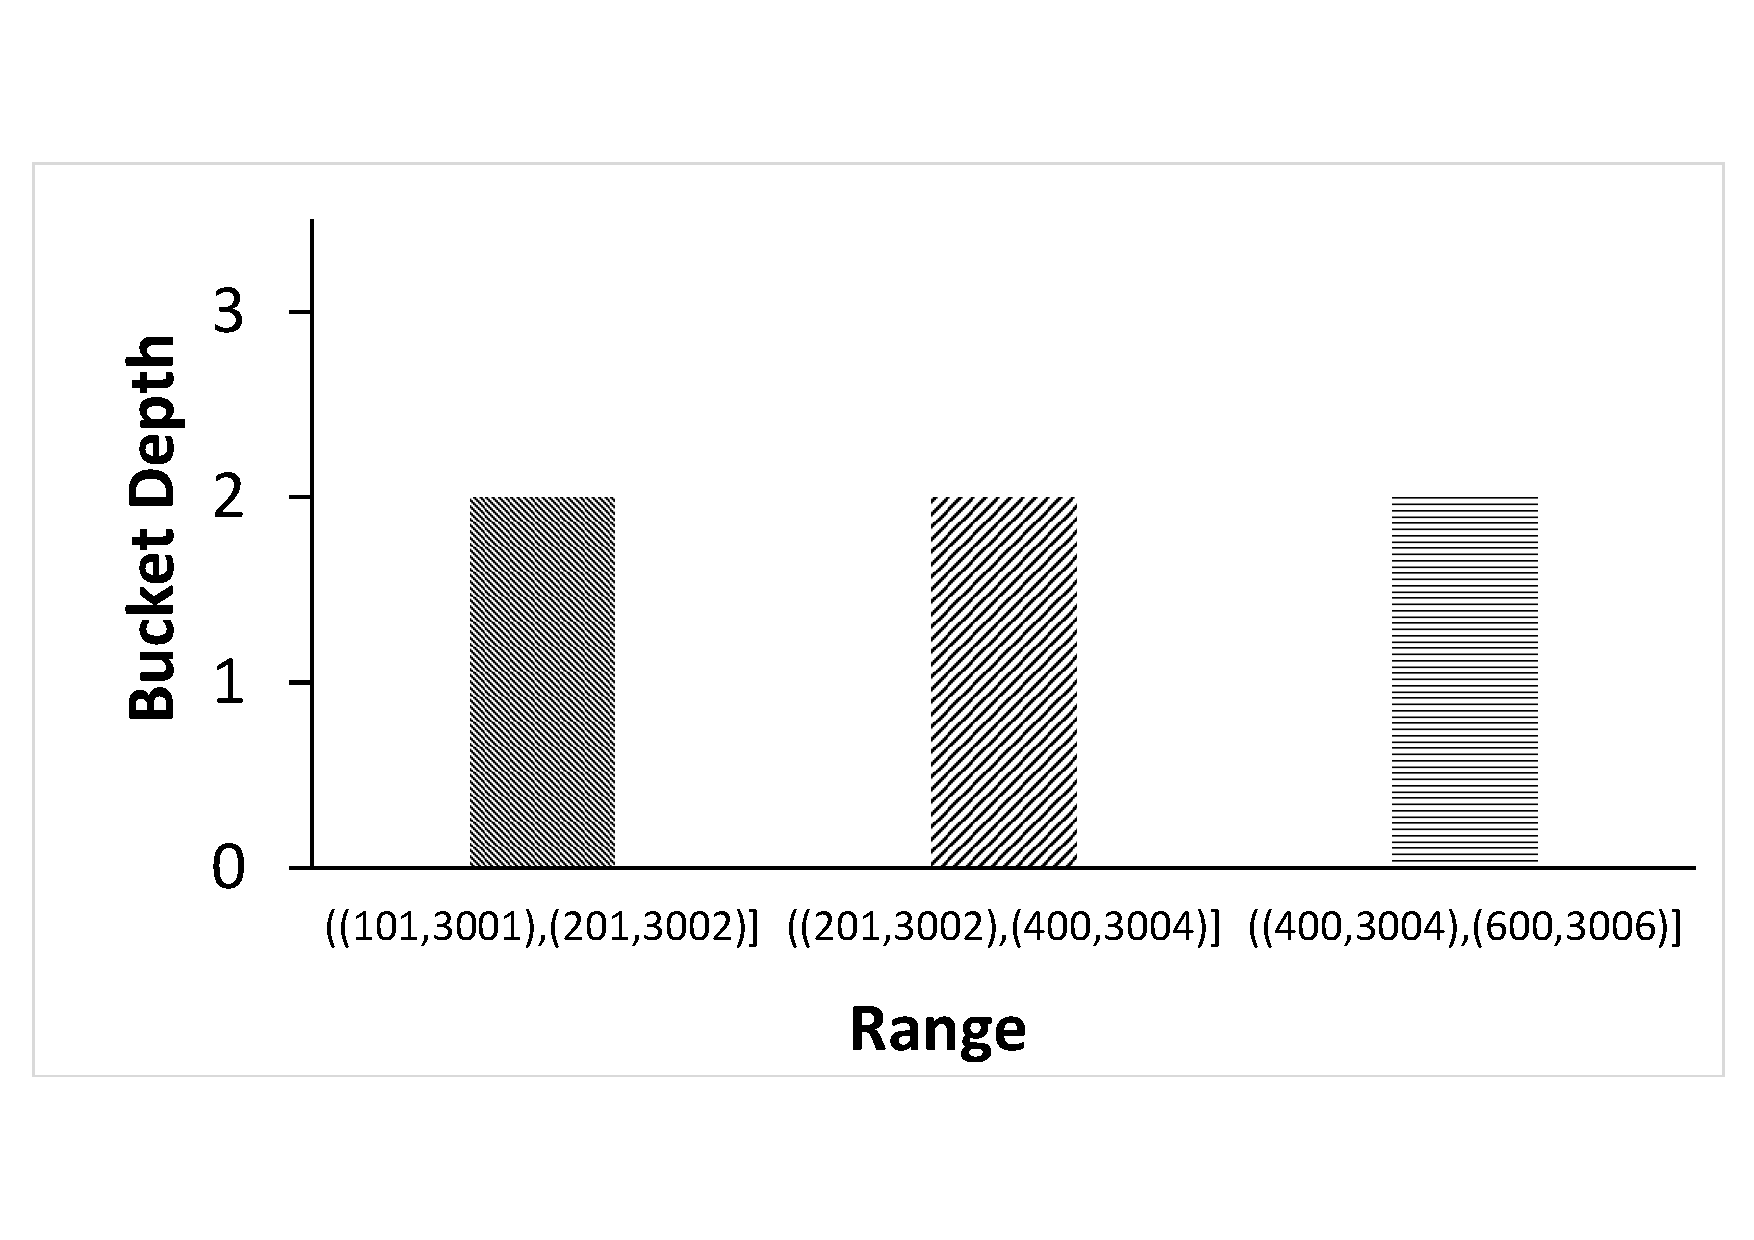
\includegraphics[width=2.4in,height=1.5in]{articlegraph/sample.pdf}
		\caption{Equal-depth Histogram}
		\label{fig:side:a}
	\end{minipage}%
	\begin{minipage}[t]{0.5\linewidth}
		\centering
		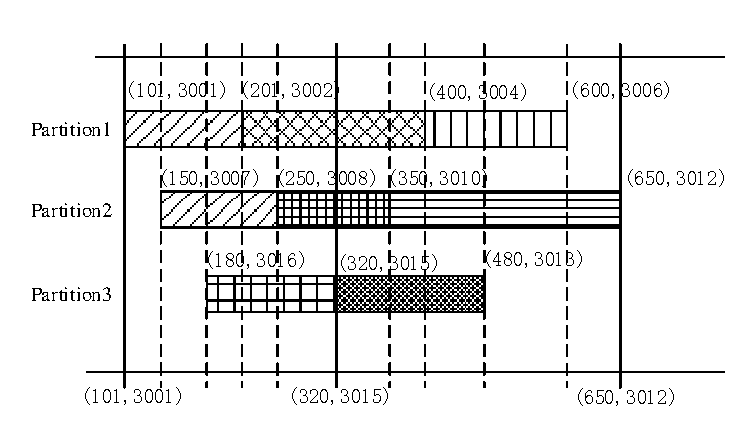
\includegraphics[width=2.6in]{articlegraph/divide.pdf}
		\caption{Partition Division}
		\label{fig:side:b}
	\end{minipage}
\end{figure}
\vspace{-0.7cm}

\begin{example}
	Take the example in Figure 4. After local index construction, the coordinator receives three histograms and will divide ranges of index partitions. The process of division is shown in Figure 6. Since the partition number of the data table is 3. For fixed-length storages, the partition  number of the index is 2. Thus, ranges of partitions are: (MIN,(320,3015)] and((320,3015),MAX). The first partition includes 7 records and the second partition includes 9 records.
\end{example}

\vspace{-0.2cm}
\subsection{Global Index Construction}
Global index construction starts after the division of index partitions. During global index construction, a data node  may receive two types of information. One is the control information from the coordinator node. Another is the data information from other data nodes. The former is the index partition construction command with a list of index partition ranges, which means the data node will maintain the index data corresponding to ranges received from the coordinator.
The latter is index records loaded from other data nodes in the given range. Certainly, the index records are sorted by the same search key. After getting all the index records in the given range, the sorted index data will be flushed to the disk serving as an index table partition.

Algorithm 4 illustrates the procedure of  global index construction. It is worth noting that Algorithm 4 must run at all data nodes received construction index messages from the coordinator. Firstly, the algorithm  prepares the data for each range according to a range list $L$ received from the coordinator (at line 4, line 8). Meanwhile, it may receive requests from other data nodes for index records and it will response to the these requests. After getting all the records of P, it will sort these records and then flush them to disk as an index partition P (at line 5, line 9). In practice, the procedure of constructing index partitions can be implemented by multi-thread technique, i.e. each range can be assigned a thread.

\SetKwProg{Fn}{\underline{Function}}{}{end}
%  \newcommand{\forcond}{$i=0$ \KwTo $n$}
\SetKwFunction{localindexconstruct}{RunLocalIndex}
\SetKwFunction{globalindexconstruct}{RunGloalIndex}
\SetKwFunction{indexrequest}{RunIndexRequest}
%\SetAlgorithmName{Figure}{}
\LinesNumbered
% \newcommand{\fortol}{$i=0$ \KwTo $L$}
% \newcommand{\fortok}{$j=1$ \KwTo $k$}
\vspace{-0.7cm}
\begin{algorithm}[!htb]
\SetAlgoLined
\caption{Global Index Construction}%
\Fn{\globalindexconstruct{$L$}}{	
  Let $P$ denote a index partition \;
   \For{each $l_i \in L$}
   {
    \If {the current data node contains all index data in range $l_i$ }
    {
    Flush index data to disk to construct index partition $P$ \;
    }
   \Else
   {
    shuffle and sort index data which is not located in current nodes with other data nodes correlated to $l_i$ \;
    %sort the index data by search key construct index partition $P$ \;
    Flush index data to disk to construct index partition $P$ \;
  }
 }

}
\end{algorithm}
\vspace{-0.7cm}

\begin{example}
Take the example of global index construction in Figure 4. After index partition division, DataNode1 receives a partition range $(MIN,(320,3015)]$ and DataNode2 receives a partition range $((320,3015),MAX]$. After getting all the records of a range,  index records are flushed to the disk serving as an index partition,  such as index partition1 and index partition2 in this example.
\end{example}

